\begin{enumerate}[label=\thesection.\arabic*.,ref=\thesection.\theenumi]
\numberwithin{equation}{enumi}
\numberwithin{figure}{enumi}
%%
\item
\label{ch4_sim}
Plot 
\begin{equation}
P_e = \pr{\hat{X} = -1|X=1}
\end{equation}
%
for 
\begin{equation}
Y = AX+N,
\end{equation}
where $A$ is Raleigh with $E\sbrak{A^2} = \gamma, N \sim \gauss{0}{1}, X \in \brak{-1,1}$ for $0 \le \gamma \le 10$ dB.
\\
\solution The estimated value $\hat{X}$ is given by
\begin{align}
\hat{X} = 
\begin{cases}
+1 & Y>0\\
-1 & Y<0
\end{cases}
\end{align}
For $X = 1$, 
\begin{align}
Y &= A + N\\
P_e &= \pr{\hat{X} = -1|X=1} \\
&= \pr{Y<0 |X=1}\\
&= \pr{A<-N}\\
&= F_A(-N)\\
&= \int_{-\infty}^{\infty} F_A(-n) \times f_N(n) dn
\end{align}
If $N>0$, $F_A(-N) = 0$. Therefore,
\begin{align}
P_e &= \int_{-\infty}^{0} F_A(-n) \times f_N(n) dn\\
&= \frac{1}{\sqrt{2\pi}}\int_{-\infty}^{0} \brak{1-\exp \left( -\frac{n^2}{2\sigma^2} \right) }\exp \left( -\frac{n^2}{2} \right) dn\\
&= \frac{1}{2\sqrt{2\pi}} \int_{-\infty}^{\infty} \exp \left( -\frac{n^2}{2} \right)dn \nonumber \\
&- \frac{1}{2\sqrt{2\pi}} \int_{-\infty}^{\infty} \exp \left( -\frac{(1+ \sigma^2)n^2}{2 \sigma^2} \right) dn\\
&= \frac{\sqrt{2\pi} - \sqrt{\frac{\pi(2\sigma^2)}{1+\sigma^2}}}{2\sqrt{2\pi}}\\
&= \frac{1}{2} - \frac{1}{2}\sqrt{\frac{\sigma^2}{1+\sigma^2}}
\end{align}
For a Rayleigh Distribution with scale $= \sigma$,
\begin{align}
E\sbrak{A^2} = 2\sigma^2\\
\gamma = 2\sigma^2\\
\therefore P_e = \frac{1}{2} - \frac{1}{2}\sqrt{\frac{\gamma}{2+\gamma}}
\end{align}
\begin{figure}
\centering
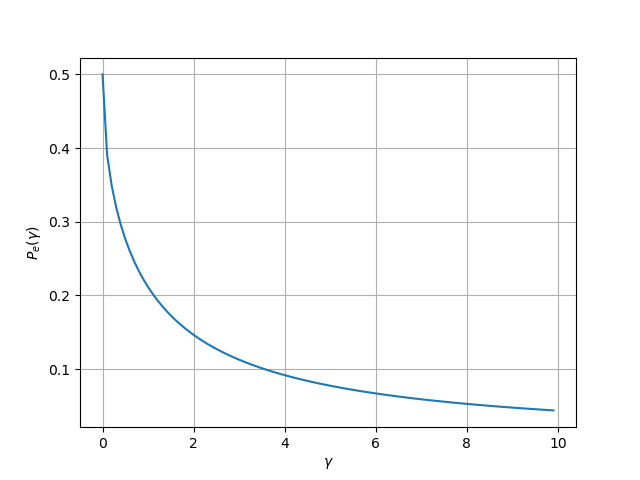
\includegraphics[width=\columnwidth]{./figs/cond/Pe_vs_gamma.png}
\caption{The value of $P_e$ for $0 \le \gamma \le 10$}
\label{fig:uni_cdf}
\end{figure}
%
\item
Assuming that $N$ is a constant, find an expression for $P_e$.  Call this $P_e(N)$

%
\item
%
\label{ch4_anal}
For a function $g$,
\begin{equation}
E\sbrak{g(X)} = \int_{-\infty}^{\infty}g(x)p_{X}(x)\, dx
\end{equation}
%
Find $P_e = E\sbrak{P_e(N)}$.

%
\item
Plot $P_e$ in problems \ref{ch4_sim} and \ref{ch4_anal} on the same graph w.r.t $\gamma$.  Comment.

\end{enumerate}
